\section{Implementation}
\label{sec:implementation}

We realize a prototype of \quark runtime for MRDTs as a lightweight
shim layer on top of Scylla -- an off-the-shelf distributed data
store~\cite{scylla}. We rely on Scylla for inter-replica
communication, data replication, persistence, and fault tolerance.
\quark translates the high-level MRDT implementations in OCaml to
their low-level representations in the backing store and orchestrates
their well-formed distributed executions.
Fig.~\ref{fig:implementation} illustrates the overall architecture.

The implementation of \quark largely follows the design of \quark
distributed machine described in Sec.~\ref{sec:concrete-sem}.  We
manifest each component of the state, namely the branch map $B$, the
value map $N$, and the head map $H$, as a column family (i.e., a
table) in Scylla. The synchronization needed to linearize merges is
implemented with help of Scylla's support for conditional updates (CAS
operations) and expiring columns. The total order among merges is
enforced with help of \C{Quorum} reads and writes. Each user process
is assigned its own branch containing a replica of the MRDT.  Version
vectors are realized as associative lists and stored in Scylla as
blobs.

\begin{figure}[ht]
  \centering
    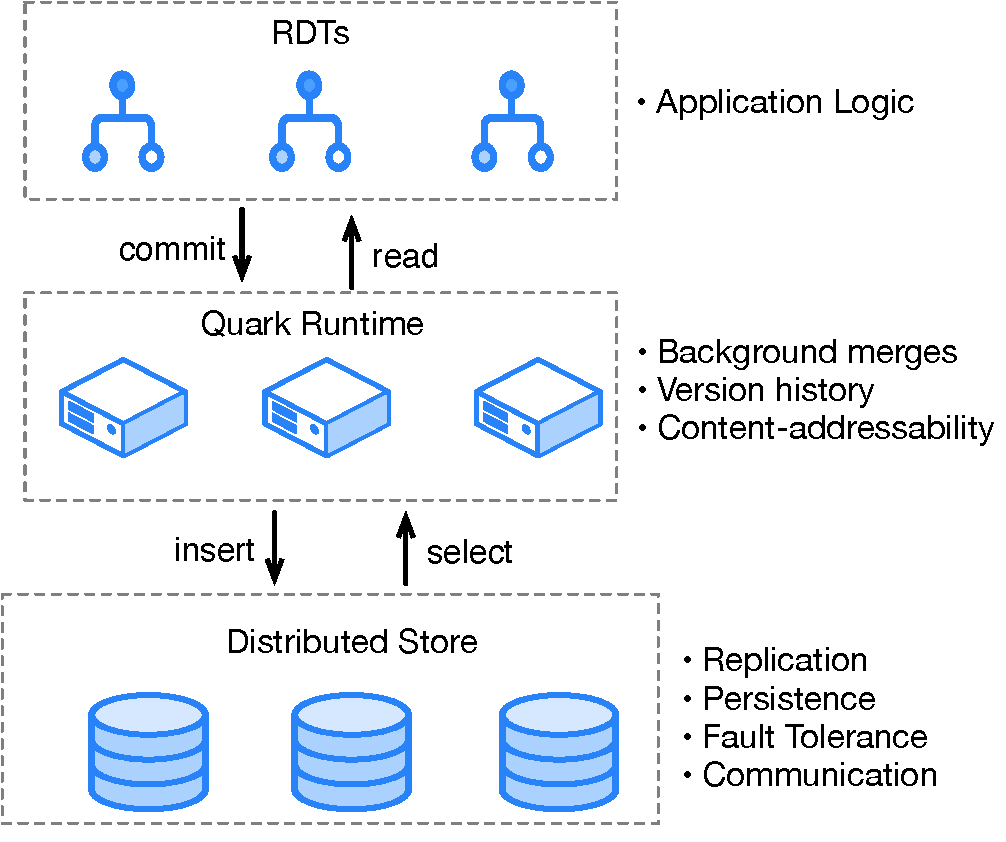
\includegraphics[scale=0.35]{Figures/implementation}
\caption{\quark implementation architecture}
\label{fig:implementation}
  \vspace*{-0.2in}
\end{figure}

The implementation however differs from the formalization in two
significant ways. First is in the treatment of MRDT values.
Formalization assumes values to be atomic with no sharing in between
them. In practice, however, an MRDT could be a linked data structure
such as a binary tree, and two such values could share a significant
amount of internal structure.  Consequently, the size of the
\emph{diff} between two consecutive versions of a value could be
asymptotically less then the size of the data structure itself, in
which case it unreasonable to transfer the entire data structure over
the network. To facilitate the efficient computation of diffs between
versions of data structures, we implement a \emph{content-addressable
store} as a key-value table in Scylla where key is simply the SHA256
hash of the value. A linked data structure is stored as a collection
of nodes, where each node links to the other by referring to its hash.
The diff between two consecutive versions of a data structure would
simply manifest as new entries in the content-addressable store
reachable from the root of the new version. The new entries, being new
data, are automatically replicated by Scylla, thus letting us
reconstruct the new version at a remote location. The root hash of the
new version is obtained from the value map $N$, which now maps version
vectors to the \emph{hashes} of values.

The second significant difference between the implementation and the
formalization is the timing of merges. Operational Semantics in
Sec.~\ref{sec:abstract-sem} and Sec.~\ref{sec:concrete-sem} interleave
commits and merges such that only one of them executes at any given
time. Since commits are initiated by the user in practice,
interleaving them with strongly consistent merges increases their
latency as perceived by the user. For the user-perceived latency to
remain unaffected, it is important that a replica be always available
to execute user requests. \quark ensures this by handling user
requests in a foreground thread that is always allowed to commit to
the local branch. Merges, on the other hand, are relegated to the
background. A background thread constantly scans the remote branches
for new versions, and if there are any, merges them into the latest
version on the local branch after checking the necessary preconditions
(Sec.~\ref{sec:abstract-sem}). 

\quark's background merges however pose a new problem as they create
new versions on the local branch in the background while a user
operation is manipulating an older version in the foreground. When
the user attempts to write their version to the store, simply
committing it would effectively override the concurrent updates from
other users obtained via background merges. The solution, fortunately,
is straightforward: \quark \emph{merges} the user-submitted version
with the latest version on the local branch to create a new version
that includes the updates from either direction. Since this merge is
fully confined to the local replica, it is guaranteed to not affect
the LCA of the local branch in relation to any remote branch. To the
external world, it appears as if the local branch has simply committed
a new version that was derived from the older version. Since the
commit operation now entails a merge, the merged version has to be
returned to the user as the result of the commit.  Consequently the
\C{write} operation exposed by \quark is a function of type
$\texttt{Value} \rightarrow \texttt{Value}$, where $\texttt{Value}$ is
any MRDT.
